 \documentclass[a4paper,12pt]{article}
\usepackage[a4paper,top=1.3cm,bottom=2cm,left=1.5cm,right=1.5cm,marginparwidth=0.75cm]{geometry}
\usepackage{setspace}
\usepackage{cmap}					
\usepackage{mathtext} 				
\usepackage[T2A]{fontenc}			
\usepackage[utf8]{inputenc}			
\usepackage[english,russian]{babel}
\usepackage{multirow}
\usepackage{graphicx}
\usepackage{wrapfig}
\usepackage{tabularx}
\usepackage{float}
\usepackage{longtable}
\usepackage{hyperref}
\hypersetup{colorlinks=true,urlcolor=blue}
\usepackage[rgb]{xcolor}
\usepackage{amsmath,amsfonts,amssymb,amsthm,mathtools} 
\usepackage{icomma} 
\mathtoolsset{showonlyrefs=true}
\usepackage{euscript}
\usepackage{mathrsfs}

\DeclareMathOperator{\sgn}{\mathop{sgn}}
\newcommand*{\hm}[1]{#1\nobreak\discretionary{}
	{\hbox{$\mathsurround=0pt #1$}}{}}


\title{\textbf{Определение моментов инерции твердых тел с помощью трифилярного подвеса. (1.2.3)}}
\author{Моргулёв Илья}
\date{Ноябрь 2023}


\begin{document}
	
	\maketitle
	
	\section{Введение}
	
	\textbf{Цели работы:} измерение момента инерции тел и сравнение результатов с расчетми по теоретиеским формулам; проверка аддитивноски моментов инерции и справедливости формулы Гюйгенса-Штейнера.\\
	\textbf{Оборудование:} трифилярный подвес, секундомер, счетчик числа колебаний, набор тел, момент инерции которых надлежит измерить (диск, стержень, полный цилиндр и другие).
	
	\section {Экспериментальная установка}
	
	\begin{wrapfigure}{l}{7cm}
		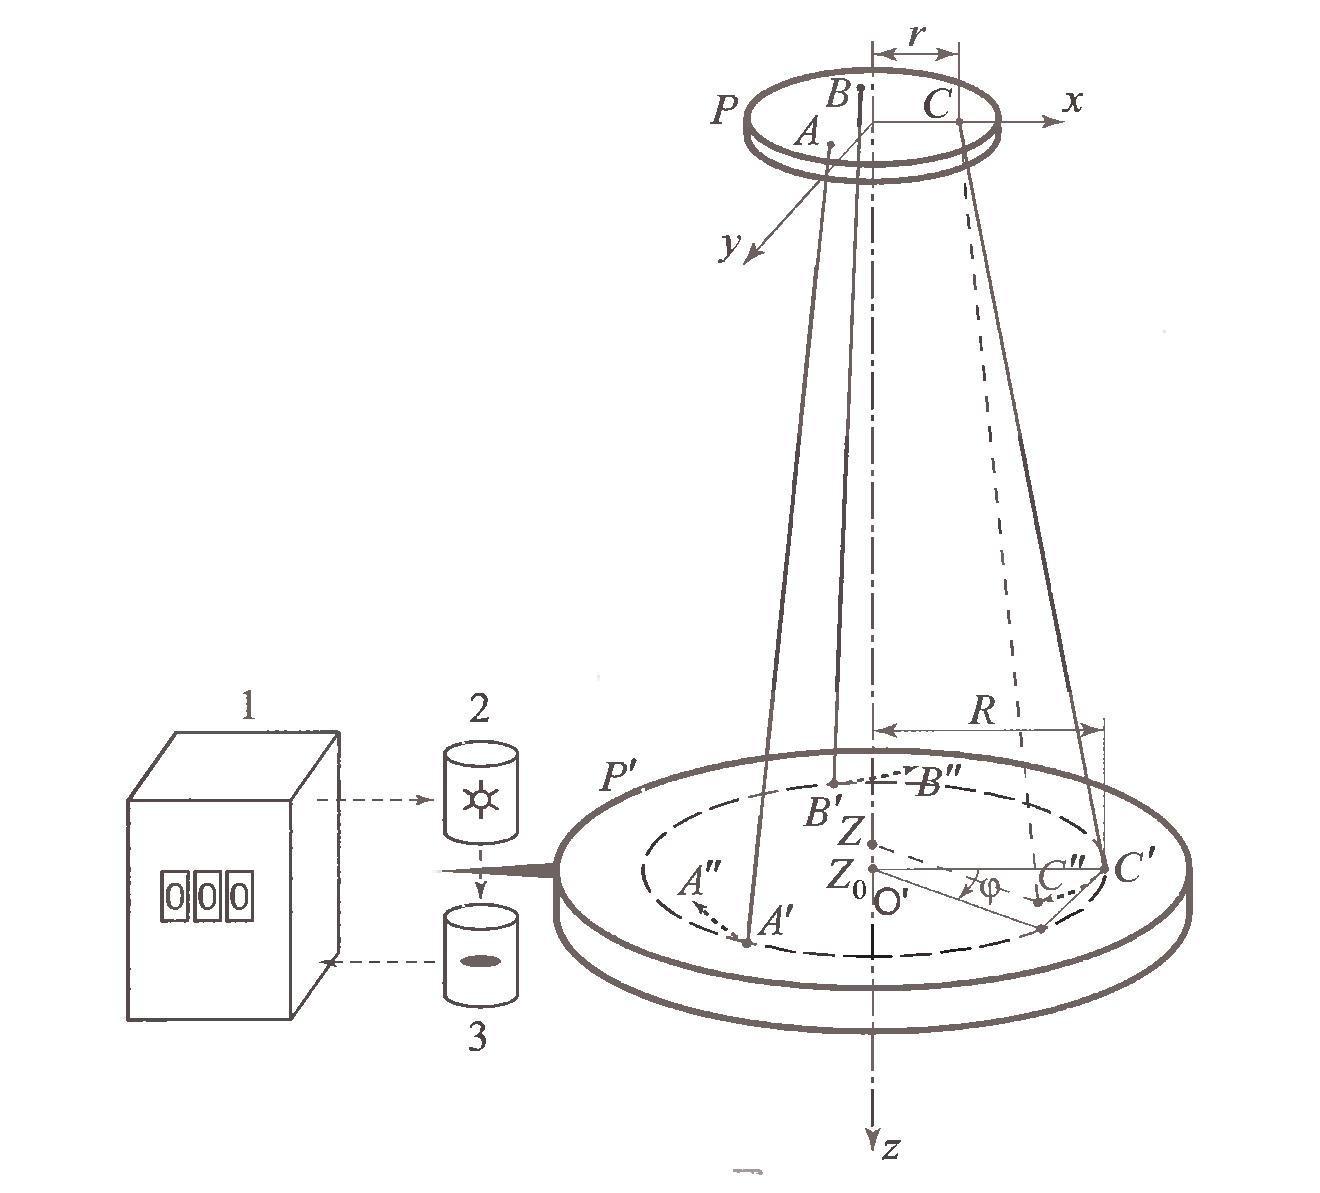
\includegraphics[width=0.95\linewidth]{1.2.3 ustan.png}
		\caption{Физический маятник}\label{risunok}
	\end{wrapfigure}
	
	Для наших целей удобно использовать устройство, показанное на Рис. \ref{risunok} и называемое трифилярным подвесом. Оно состоит из укрепленной на некоторой высоте неподвижной платформы $P$ и подвешенной к ней на трех симметрично расположеных нитях $AA'$, $BB'$ и $CC'$, вращающейся платформы $P'$. 
	
	Чтобы не вызывать дополнительных раскачиваний, лучше поворачивать верхнюю платформу, укрепленную на неподвижной оси. После поворота верхняя платформа остается неподвижной в течение всего процесса колебний. После того, как нижняя платформа $P'$ оказывается повернутой на угол $\varphi$ относительно верхней платформы $P$, вощникает момент сил, стремящийся вернуть нижнюю платформу в положение равновесия, при котором относительный поворот платформ отсутствует. В результате платформа совершает крутильные колебания.
	
	\section{Теоретические сведения}
	
	\par Инерционность при вращении тела относительно оси определяется моментом инерции тела относительно этой оси. Момент инерции твердого тела относительно неподвижной оси вращения вычисляется по формуле:
	
	\begin{equation}
		I = \int r^2 dm
	\end{equation}
	
	Здесь $r$ -- расстояние элемента массы тела $dm$ от оси вращения. Интегрирование проводится по всей массе тела $m$.
	
	Если пренебречь потерями энергии на трение о воздух и крепление нитей, то уравнение сохранения энергии при коебаниях можно записать следующим образом:
	
	\begin{equation}\label{moment}
		\frac{I \dot{\varphi^2}}{2} + mg(z_0-z) = E
	\end{equation}
	
	Здесь $I$ -- момент инерции платформы вместе с исследуемым телом, $m$ -- масса платформы с телом, $\varphi$ -- угол поворота платформы от положения равновесия системы, $z_0$ -- координата по вертикали центра нижней платформы $O'$  при равновесии ($\varphi = 0$), $z$ -- координата той же точки при некотором угле поворота $\varphi$. Превый член в левой части уравнения -- кинетическач энергия вращения, второй член -- потенциальная энергия в поле тяжести, $E$ -- полная энергия системы (платформы с телом).
	
	Воспользуемся системой координат $x, y, z$, связанной с верхней платформой, как показано на Рис. \ref{risunok}. Координаты верхнего конца одной из нитей подвеса точки $C$ в этой системе -- $(r, 0, 0)$. Нижний конец данной нити $C'$, находящийся на нижней платформе, при равновесии имеет координаты $(R, 0, z_0)$, а при повороте платформы на угол $\varphi$ эта точка переходит в $C''$ с координатами $(Rcos\varphi, Rsin\varphi, z)$. расстояние между точками $C$ и $C''$ равно длине нити, поэтому, после некоторых преобразований, получаем: 
	
	\begin{center}
	\begin{spacing}{1.6}
		$ (R\cos\phi - r)^2 + R^2\sin^2\phi + z^2 = L^2 $
		
		$ z^2 = L^2 - R^2 - r^2 + 2Rr\cos\phi \approx z^2_{0} - 2Rr(1 - \cos\phi) \approx z^2_{0} - Rr\phi^2 $
		
		$ z = \sqrt{z^2_{0} - Rr\phi^2} \approx z_{0} - \frac{Rr\phi^2}{2z_{0}} $
	\end{spacing}
	\end{center}

	Подставляя $z$ в уравнение \eqref{moment}, получаем:
	
	\begin{equation}
		\frac{1}{2}I\dot{\varphi^2} + mg \frac{Rr}{2z_0}\varphi^2 = E
	\end{equation}
	
	Дифференцируя по времени и сокращая на $\dot\varphi$, находим уравнение крутильных колебаний системы:
	
	\begin{equation}
		I\ddot\varphi^2 + mg\frac{Rr}{2z_0}\varphi^2 = 0
	\end{equation}
		
	Производная по времени от $E$ равна нулю, так как потерями на трение, как уже было сказано выше, пренебрегаем.
	
	Решение этого уравнения имеет вид:
	
	\begin{equation}
		\varphi = \varphi_0 sin \left(\sqrt{\frac{mgRr}{Iz_0}}t + \theta\right)
	\end{equation}

	Здесь амплитуда $\varphi_0$ и фаза $\theta$ колебаний определяются начальными условиями. Период кртуильных полебаний нашей системы равен:
	
	\begin{equation}
		T = 2\pi \sqrt{\frac{Iz_0}{mgRr}}
	\end{equation}

	Из формулы для периода получаем:
	
	\begin{equation}\label{momin}
		I = \frac{mgRrT^2}{4 \pi^2z_0} = kmT^2
	\end{equation}
	\noindent где $k = \frac{gRr}{4\pi^2z_0}$ -- величина, постоянная для данной установки.
	
	\section{Задание}
	\subsection{Проверка установки}
	При возбуждении крутильных колебаний маятникообразных движений платформы не наблюдается -- устройство функционирует нормально.
	
	При выводе формул мы предполагали, что потери энергии, связанные с трением, малы, то есть мало затухание колебаний. Это значит, что теоретические вычисления будут верны, если выполняется условие:
	
	\begin{equation}
		\tau \gg T
	\end{equation}
	
	Проверим данное условие. При отклонении на угол $\alpha \approx 5^\circ$ время, закоторое амплитуда уменьшится в 2 раза, $\tau \approx 300\text{ с}$, а $T \approx 3,5\text{ с}$. Соотношение выполняется -- установка пригодна для проведение эксперимента. Начальное отклоненеи было выбрано $\alpha \approx 5^\circ$.
	
	\subsection{Параметры установки и коэффицент $k$}
	
	Работа выполнялась на установке №6, ее параметры указаны в Таблице \eqref{param}
	\begin{table}[H]
	\begin{center}
		\begin{tabular}{|c|c|c|c|c|}
			\hline
			$m \text{, г}$  & $R\text{, мм}$ & $r\text{, мм}$ & $L\text{, см}$ & $z_0\text{, см}$\\
			\hline
			983,2 & 114,6 & 30,5 & 215,2 & 215\\
			\hline
			\hline
			$\sigma_m \text{, г}$  & $\sigma_R\text{, мм}$ & $\sigma_r\text{, мм}$ & $\sigma_L\text{, см}$ & $\sigma_{z_0}\text{, см}$\\
			\hline
			0,5 & 0,5 & 0,3 & 0,1 & 0,1\\
			\hline 
		\end{tabular}
	\caption{Парметры установки}
	\label{param}
	\end{center}
	\end{table}

	\noindent где $\sigma_m$, $\sigma_R$, $\sigma_r$, $\sigma_L$, $\sigma_{z_0}$ -- погрешности соответсвующих величин.
	
	\bigskip

	По полученным данным вычислим постоянную для конструкции №6:
	
	\begin{equation}
		k = \frac{gRr}{4\pi^2z_0} \approx 4,12\cdot 10^{-4} \frac{\text{м}^2}{\text{с}^2}
	\end{equation}

	Погрешность же $k$ будет равна:
	 
	\begin{equation}
	 	\sigma_k = k \cdot \sqrt{\left( \frac{\sigma_R}{R}\right)^2 + \left( \frac{\sigma_r}{r}\right)^2 + \left( \frac{\sigma_{z_0}}{z_0}\right)^2} \approx 0,044 \cdot 10^{-4} \frac{\text{м}^2}{\text{с}^2}
	\end{equation}
	 
	\subsection{Момент инерции платформы}
	 
	Определить момент инерции платформы можно по формуле \eqref{momin}. Для этого нам необходимо определить период колебаний ненагруженной платформы. Измеряем преиод, получаем:
	
	\begin{table}[!h]
		\begin{center}
			\begin{tabular}{|c|c|c|c|}
				\hline
				№ & Количество полных колебаний & Время колебаний -- $t_n \text{, с}$ & Период колебаний -- $T\text{ с}$\\
				\hline
				1 & \multirow{3}{*}{20} & 87,245 & 4,3623\\
				\cline{1-1} \cline{3-4}
				2 &  & 87,244 & 4,3622\\
				\cline{1-1} \cline{3-4}
				3 & & 87,251 & 4,3626\\
				\hline
			\end{tabular}
		\end{center}
	\end{table}
	
	Тогда, средний период колебания платформы будет: $T_\text{ср} \approx 4,3624\text{ с}$
	
	Давайте здесь же и определим погрешность времени: 
	
	\begin{equation}
		\sigma_T^{\text{сист}} = 0,015\text{ с}
	\end{equation}
	\begin{equation}
		\sigma_T^{\text{случ}} = \sigma_\text{случ}=\sqrt{\frac{1}{  N_\text{изм} \left( N_\text{изм} - 1 \right)}\sum_{i=1}^{N_\text{изм}}\left( T_\text{ср} - T_i \right)^2 } \approx 1,2\cdot 10^{-4}\text{, c}
	\end{equation}
	\begin{equation}
		\sigma_T = \sqrt{\sigma_\text{случ}^{2} + \sigma_{\text{сист}}^{2}} \approx 0,015\text{ с}
	\end{equation}
	Значит $T_\text{ср} = \left(4,396 \pm 0,015\right)\text{ с}$. Теперь мы можем определить момент инерции платформы:
	
	\begin{equation}
			I_\text{пл} = kmT^2 \approx 7,71  \text{ кг $\cdot$ $\text{м}^2$ $\cdot 10^{-3}$}  
	\end{equation}

	Найдем погрешность найденного нами момента инерции платформы:
	
	\begin{equation}
		\varepsilon_I = \sqrt{ \left(\frac{\sigma_k}{k}\right)^2 +\left(\frac{\sigma_m}{m}\right)^2 + \left(2\frac{\sigma_T}{T}\right)^2} \approx 0,012
	\end{equation}
	\begin{equation}
		\sigma_{I_\text{пл}} = \varepsilon_I \cdot I_\text{пл} \approx 0,098 \text{  кг $\cdot$ $\text{м}^2$ $\cdot 10^{-3}$}
	\end{equation}
	Получаем, что с помощью данной конструкции мы можем определять момент инерции тела с погрешностью 1\%, и $I_\text{пл} = \left(7,71 \pm 0,098\right) \text{,  кг $\cdot$ $\text{м}^2$ $\cdot 10^{-3}$}$
	
	\subsection{Определение моментов инерции различных тел. Аддитивность моментов инерции}
	
	Измерим периоды колебаний платформы с различными телами таким же образом, как и для ненагруженной платформы, а именно -- 3 измерения по 20 колебаний для каждого набора тел, получаем:
	
	\begin{table}[!h]
		\begin{center}
			\begin{tabular}{|c|c|c|c|c|}
				\hline
				Набор тел & $t_0$, с & $T_0$, с & $m_0$, г & Момент инерции, кг$\cdot \text{м}^2 \cdot 10^{-3}$\\
				\hline
				Платформа& 87,244 & 4,3624 & 983,2 & 7,71\\
				\hline
				Платформа + диск  & 38,958 & 3,8958 & 1573 & 9,836  \\
				\hline
				Платформа + кольцо   & 41,444 & 4,1444 & 1760,1 & 12,455 \\
				\hline
				Платформа + кольцо + цилиндр &   38,871 & 3,8871 & 2349,9 & 14,628 \\
				\hline
			\end{tabular}
		\caption{Моменты инерции платформы с различными телами}
		\label{momtel}
		\end{center}
	\end{table}
	
	Для подтверждения аддитивности необходимо показать,что выполняются условия:
	
	
		\begin{equation} \label{plc}
			I_\text{пл+ц} = I_\text{пл} + I_\text{ц}
		\end{equation}
		\begin{equation}\label{plk}
			I_\text{пл+к} = I_\text{пл} + I_\text{к}
		\end{equation}
		\begin{equation}
			I_\text{пл+ц+к} = I_\text{пл} + I_\text{ц} + I_\text{к}
			\label{plck}
		\end{equation}
	
	
	Из Таблицы \eqref{momtel} и формул \eqref{plc}, \eqref{plk} мы можем найти момент инерции диска и кольца: $I_\text{д} = I_\text{пл+д} - I_\text{пл} = \left(2,126 \pm 0,122\right) \text{ кг $\cdot$ $\text{м}^2$ $\cdot 10^{-3}$}$, а $I_\text{к} = I_\text{пл+к} - I_\text{пл} = \left(4,745 \pm 0,161\right) \text{ кг $\cdot$ $\text{м}^2$ $\cdot 10^{-3}$}$. 
	
	Тогда, для доказательства аддитивности, проверим уравнение \eqref{plck}. Оно выполняется, следовательно моменты инерции аддитивны.
	
	Теперь сравним полученные нами моменты инерциии для тел, и их теоретические значения. Для диска момент инерции вычисляется следующим образом: $I_\text{д} = \frac{1}{2}m_\text{д}R_\text{д}^2$. Радиус данного диска $R_\text{д} = 8,46 \text{ см}$, тогда $I_\text{д} = 2,111 \text{  кг $\cdot$ $\text{м}^2$ $\cdot 10^{-3}$}$, что подтверждает экспериментальное значение.
	
	Для кольца же: $I_\text{к} = m_\text{к}R_\text{к}^2$. Так как данное кольцо не идеально тонко, то $R_\text{к} = \frac{D_\text{внут} + h}{2}$, где $h = 0,32 \text{, см}$, а $D_\text{внут} = 14,29\text{ см}$, тогда $R_\text{к} = 7,8 \text{ см}$. Получаем, что $I_\text{к} = 4,726\text{  кг $\cdot$ $\text{м}^2$ $\cdot 10^{-3}$}$, что тоже совпадает с полученным экспериментально значением.
	
	\subsection{Зависимость момента инерции системы тел от их расположения. График зависимости $I(h^2)$}
	
	\begin{wrapfigure}[10]{r}{0.29\textwidth}
		\vspace{-3em}
		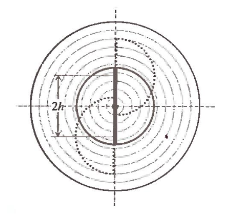
\includegraphics[width=0.25\textwidth]{position}
		\caption{Схема расположения грузов на платформе трифилярного подвеса.}
		\label{ris:position}
	\end{wrapfigure}
	
	Определим зависимость момента инерции системы двух тел от их взаимного расположения. Для этого располагая грузы, как показано на рис. \ref{ris:position}, получим зависимость от расстояния. Затем Используя формулу \ref{momin}, определим зависимость $I(h^2)$.
	
	Полученные результаты измерений занесем в таблицы \eqref{tab:period},\eqref{tab:moment} соответсвенно. Основывыаясь на результатах таблицы \eqref{tab:moment}, построим график зависимости $ I(h^{2}) $ (Рис. \ref{ris:grafik}).
	\bigskip\bigskip\bigskip\bigskip\bigskip
	
	\begin{table}[!h]
		\begin{center}
			\begin{tabular}{| c | c | c || c | c | c |}
				\hline
				№ изм. & T, с & h, см & № изм. & T, с & h, см \\ \hline
				1 & 3,055 & 0 & 8 & 3,336 & 3,5 \\ \hline
				2 & 3,063 & 0,5 & 9 & 3,417 & 4,0 \\ \hline
				3 & 3,078 & 1,0 & 10 & 3,511 & 5,5 \\ \hline
				4 & 3,113 & 1,5 & 11 & 3,607 & 5,0 \\ \hline
				5 & 3,154 & 2,0 & 12 &  &  \\ \hline
				6 & 3,196 & 2,5 & 13 &  &  \\ \hline
				7 & 3,267 & 3,0 & 14 &  &  \\ \hline
				
			\end{tabular}
			\caption{Зависимость Периода колебаний от расстояния}
			\label{tab:period}
		\end{center}
	\end{table}
	\begin{table}[!h]
		\begin{center}
			\begin{tabular}{| c | c | c || c | c | c |}
				\hline
				№ изм. & I $\text{,  кг $\cdot$ $\text{м}^2$ $\cdot 10^{-3}$}$ & h, cm & № изм. & I $\text{,  кг $\cdot$ $\text{м}^2$ $\cdot 10^{-3}$}$ & h, сm \\ \hline
				1 & 9,327 & 0 & 8 & 11,123 & 3,5 \\ \hline
				2 & 9,377 & 0,5 & 9 & 11,669 & 4,0 \\ \hline
				3 & 9,467 & 1,0 & 10 & 12,320 & 5,5 \\ \hline
				4 & 9,685 & 1,5 & 11 & 13,003 & 5,0 \\ \hline
				5 & 9,942 & 2,0 & 12 &  &  \\ \hline
				6 & 10,209 & 2,5 & 13 &  &  \\ \hline
				7 & 10,667 & 3,0 & 14 &  &  \\ \hline
			\end{tabular}
			\caption{Зависимость момента инерции системы от расстояния}
			\label{tab:moment}
		\end{center}
	\end{table}
	
	\begin{figure}[!h]
		\begin{center}
			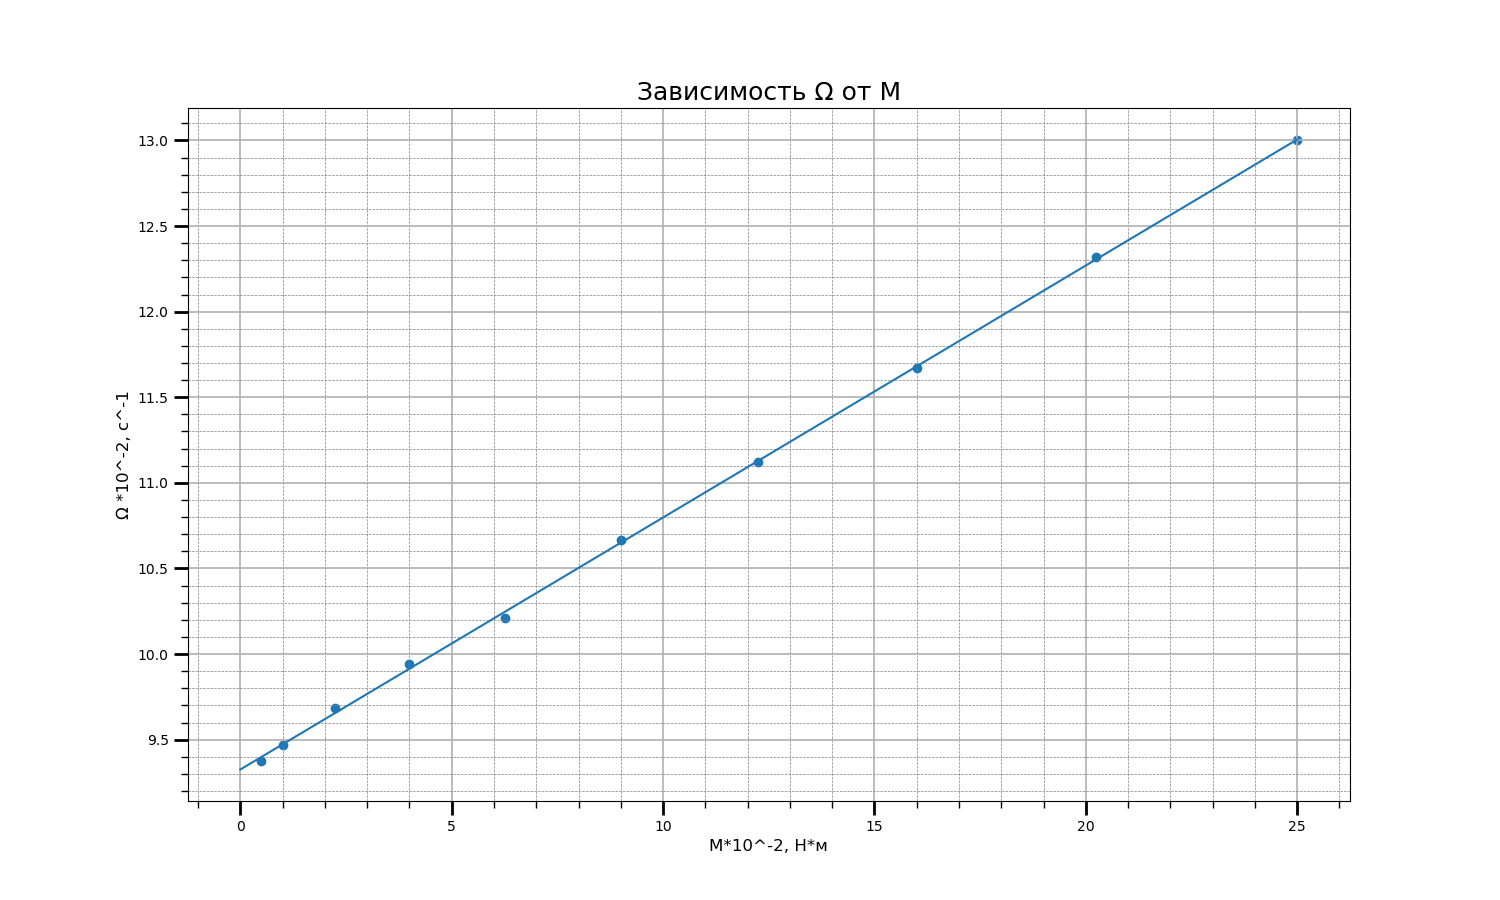
\includegraphics[width=0.9\textwidth]{graf.png}
			\caption{График зависимости $ I(h^2) $}
			\label{ris:grafik}
		\end{center}
	\end{figure}
	
	По графику понятно, что $I = kh^2 + b$. Тогда $b$ -- момент инерции платформы + диска. Для вычисления коэффициентов $ k $ и $ b $ воспользуемся методом наименьших квадратов:
	
	\begin{equation}
		k=\frac{\langle xy\rangle-\langle x\rangle \langle y\rangle}{\langle x^2\rangle - \langle x\rangle^2}\approx 0,1472 \frac{\text{кг}\cdot\text{м}^2}{\text{см}^2}\cdot 10^{-3},
	\end{equation}
	
	\begin{equation}
		b=\langle y \rangle -k\langle x \rangle\approx 9,3255\text{  кг $\cdot$ $\text{м}^2$ $\cdot 10^{-3}$},
	\end{equation}
	где $ x=h^2 $, $ y=I $.
	
	Случайные погрешности вычисления $ k $ и $ b $ можно найти по следующим формулам:
	
	\begin{equation}
		\sigma_k^\text{случ}=\frac{1}{\sqrt{N}}\sqrt{\frac{\langle y^2 \rangle - \langle y \rangle^2}{\langle x^2 \rangle - \langle x \rangle^2} - k^2  } \approx 0,0007 \frac{\text{кг}\cdot\text{м}^2}{\text{см}^2}\cdot 10^{-3},
	\end{equation}
	
	\begin{equation}
		\sigma_b^\text{случ}= \sigma_k^\text{случ} \sqrt{\langle x^2 \rangle - \langle x \rangle^2} \approx 0,006 \text{  кг $\cdot$ $\text{м}^2$ $\cdot 10^{-3}$}.
	\end{equation}
	
	Систематическая погрешность вычисления коэффициентов определяется следующим соотношением:
	
	\begin{equation}
		\sigma^\text{сист}_b = b\sqrt{\left( \varepsilon_{I} \right)^2 + \left( \varepsilon_{h^2} \right)^2 } \approx b \cdot \varepsilon_I \approx 0,118 \text{  кг $\cdot$ $\text{м}^2$ $\cdot 10^{-3}$}.
	\end{equation}
	
	Тогда полную погрешность вычисления коэффициентов подсчитываем по следующей формуле:
	
	\begin{equation}
		\sigma_b = \sqrt{\left( \sigma_b^\text{случ} \right)^2 + \left( \sigma_b^\text{сист} \right)^2 } \approx 0,118 \text{  кг $\cdot$ $\text{м}^2$ $\cdot 10^{-3}$}.
	\end{equation}
	
	Необходимый нам момент инерции можно найти при $h = 0$, тогда $b = I_\text{пл+д} = I_\text{пл} + I_\text{д} = \left(9,327 \pm 0,118 \right) \text{  кг $\cdot$ $\text{м}^2$ $\cdot 10^{-3}$}$. Так как момент инерции платформы уже изветсен, и он равняется: $I_\text{пл} = \left(7,71 \pm 0,098 \right) \text{  кг $\cdot$ $\text{м}^2$ $\cdot 10^{-3}$}$, то момент инерции диска \underline{$I_\text{д} = \left(1,617 \pm 0,141 \right) \text{  кг $\cdot$ $\text{м}^2$ $\cdot 10^{-3}$}$}.
	
	Зная радиус диска $R_\text{д} = (0,0473 \pm 0,0001)$ м, мы можем определить его массу: $m_\text{д} = 2I_\text{д}/R_\text{д}^2 \approx 1,4455$ кг, $\sigma_{m_\text{д}} = m_\text{д} \cdot \sqrt{\varepsilon_I^2+\left(2\varepsilon_R\right)^2} \approx  0,126$, кг. Значит, что экспериментальная масса диска \underline{$m_\text{д} = \left(1,4455 \pm 0,126 \right)\text{ кг}$}, что совпадает с реальной полной массой диска $m = (1442,6 \pm 0,1)\text{ г}$. 
	
	\section{Вывод}
	
	С помощью трифилярного подвеса можно определять момент инерции с достаточно большой точностью $\varepsilon \approx 1,3\%$. Такая точность обусловлена малой погрешностью измерения времени и условиями, при которых колебания подвеса можно считать слабозатухающими.
	
	Мы экспериментально доказали аддитивность моментов инерции с помощью различных тел и подтвердили действие теоремы Гюйгенса.
	
	Полученная зависимость $I(h^2)$ аппроксимируется линейой зависимостью, что подвтерждает формулу Гюйгенса-Штейнера ($I = I_c + Mh^2$, где $I$ -- момент инерции тела, $I_c$ --момент инерции тела относительно центра, $M$ -- масса тела, а $h$ -- расстояние между двумя осями, в нашем случае -- между осью вращения и половинками диска).
	
	
\end{document}
